\section{Convergenza globale del metodo di Newton ("delle tangenti") in ipotesi di convessità/concavità stretta}
\underline{Metodo di Newton}: Linearizzare iterativamente la funzione con la tangente nel punto
\[
\begin{cases}
	y = 0 \\
	y = f(x_n) + f'(x_n)(x-x_n) 
\end{cases}
\Rightarrow \,\,\,\,x_{n+1} = x_n - \frac{f(x_n)}{f'(x_n)}
\]
\underline{Convergenza metodo di Newton}:\\
\[
\begin{cases}
	f\in C^2[a,b]\\
	f(a)f(b)<0\\
	f''(x)>0 \,\,\,\,\, \forall x\in [a,b]\\
	x_0 : f(x_0)f''(x_0)>0
\end{cases}
\Rightarrow \underset{\text{e converge all'unico zero $\xi$ di $f$ in $[a,b]$}}{\text{Il metodo di Newton è ben definto (cioè $f'(x_n)\ne 0$)}}
\]
\textbf{Dimostrazione}\\
ci sono 4 casi possibili in base al segno di $f''$ ovvero
\begin{center}
	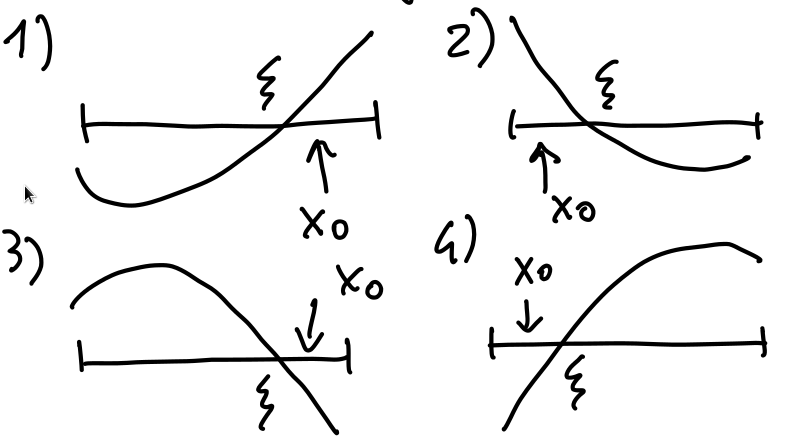
\includegraphics[scale=0.35]{pagina11_1.png}
\end{center}
In questa dimostrazione di concentriamo sul caso 1)\\
\begin{center}
	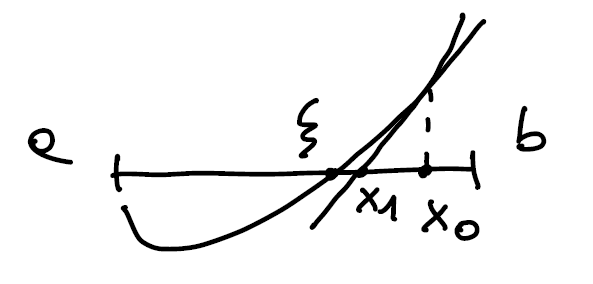
\includegraphics[width=0.3\textwidth]{pagina12_2.PNG} 
\end{center}
\begin{itemize}
	\item $f(a)<0\,,\, f(b)>0$
	\item $f''(x)>0\,\,\, \forall x\in [a,b]$
	\item $x_0\in [a,b]$
\end{itemize}
Dimostriamo come prima cosa: $x_n\in (\xi,b] \Rightarrow x_{n+1}\in (\xi,b]$
\begin{center}
	$f$ è esattamente convessa $\Rightarrow$ La tangente sta "sotto al grafico" $\forall x\in [a,b]$ \\$\Rightarrow $ La tangente in un punto $\in (\xi,b]$ interseca l'asse $x$ "a destra" di $\xi$
\end{center}
Dimostriamo quindi: $x_{n+1}<x_n$ (cioè $\{x_n\}$ è decrescente) 
\[
x_{n+1} = x_n - 
\begin{rcases}
\frac{f(x_n)}{f'(x_n)}
\end{rcases}
>0
\]
Poiché per $x_n \in (\xi,b\,]$ si ha $f(x_n)>0$. Inoltre $f'(x_n)>0$ in $(\xi,b\,]$ altrimenti per avere uno zero $f''$ in $(\xi,b\,]$ dovrebbe cambiare segno.\\
Abbiamo quindi che $\{x_n\}$ è una successione decrescente, con $x_n>\xi \,\,\,\,\, \forall n$.\\
Allora
\[
\exists \lim_{n \to \infty} x_n = inf\{x_n\} = \eta \quad \text{con} \quad \eta \geq \xi\
\]
Infine
\[
\begin{split}
\eta & = \lim x_{n+1} = \lim \left( x_n - \frac{f(x_n)}{f'(x_n)} \right) \\
& = \lim x_n - \lim\frac{f(x_n)}{f'(x_n)} \\
& = \lim x_n - \frac{\lim f(x_n)}{\lim f'(x_n)} \\ 
& = \lim x_n - \frac{f(\lim x_n)}{f'(\lim x_n)} \leftarrow \,\, \lim x_n=\eta\\
& = \eta - \frac{f(\eta)}{f'(\eta)}
\end{split}
\]
Quindi
\[\eta=\eta-\frac{f(\eta)}{f'(\eta)} \quad \text{ con } f'(\eta) \neq 0 \Rightarrow \frac{f(\eta)}{f'(\eta)} = 0 \Rightarrow f(\eta)=0 \Rightarrow \eta=\xi\]



